\documentclass{article}
\usepackage{spconf,amsmath,graphicx}

% It's fine to compress itemized lists if you used them in the
% manuscript
\usepackage{enumitem}
\setlist{nosep, leftmargin=14pt}

\usepackage{minted}
\usepackage{xurl}
\usepackage{xcolor}
\usepackage{hyperref}
\usepackage{booktabs}

\hypersetup{
    colorlinks,
    linkcolor={black},
    citecolor={green!50!black},
    urlcolor={blue!80!black}
}

\definecolor{lightgray}{gray}{0.95}
\setminted{bgcolor=lightgray,breaklines,breakanywhere}

\title{Reproducing REPA}

\name{
  \begin{tabular}{@{}c@{}}
    Frederik Kraglund (\texttt{fpk297}) \qquad 
    Mark Mizzi (\texttt{rtd992}) \qquad 
    Natasha Hallberg (\texttt{gpk607}) \\
    Ondrej Varga (\texttt{wbz810})
  \end{tabular}
}

\address{
  ATDL Group 19, Department of Computer Science, University of Copenhagen
}

\begin{document}

\maketitle

\begin{abstract} 
De-noising models are expensive to train as they have to learn semantics from scratch before they can generate meaningful images. Previous work shows that regularizing the training process by aligning a projection of an intermediate hidden layer with features sourced from pre-trained encoders yields a substantial improvement in generation quality. In this work, we present a reproduction of some of the results from representation alignment (REPA) paper which originally proposed this technique.\footnote{Our work is therefore a part of the replication track.} Specifically, we investigate how generation quality is affected by changes in encoder family, trained model size, training duration, and representation-matching depth. Our results confirm that all four decisions affect generative quality and largely agree with the published numbers. 

\end{abstract}

\section{Introduction}
%I changed this section slightly to make it flow with the abstract and simultaniously make it less ambiguous; Frederik
This project aims to reproduce the results in REPA~\cite{yu2025repa}, specifically selected parts of Tables 2 and 3. We believe replicating the main findings of this paper is important as certain design choices are assumed to be generally optimal and are inherited in subsequent works (e.g. REG~\cite{wu2025representationentanglementgenerationtraining}), such as a representation-matching depth of eight, which~\cite{yu2025repa} claim is optimal.  

%~\cite{wu2025representationentanglementgenerationtraining,zheng2025diffusiontransformersrepresentationautoencoders,bolya2025perceptionencoderbestvisual,geng2025meanflowsonestepgenerative}.

\section{Theoretical Background}\label{sec:theory}

Diffusion models have arisen as a powerful generative modelling framework for creating data from noise by gradually denoising a noise image given as input~\cite{ho2020ddpm}. Such models learn to generate new data by reversing a learned data corruption process which consists of adding more and more noise to clean data samples. More recently, diffusion models shifted from originally proposed U-Net architectures~\cite{ronneberger2015unet} towards transformer backbones. In particular, \cite{yu2025repa} uses DiT (Diffusion Transformer~\cite{peebles2023dit}) and SiT (Scalable Interpolant Transformer~\cite{sit}) for diffusion and flow-matching generative modelling respectively.

Another actively developing area is representation learning. Recent strong self-supervised visual encoders such as DINOv2~\cite{oquab2023dinov2} map images to embedding vectors of rich semantic features. Those can be used in many downstream tasks, for e.g. by training a small task-specific head on top of image embeddings to do classification, segmentation etc.

The idea of REPA is to utilize rich embeddings learned by models like DINOv2 during the diffusion generative process. One assumption behind REPA is that during training, diffusion models have to learn both semantic features of images and the image corruption process simultaneously. Helping them with one of the tasks, namely with learning semantic features, should therefore speed up training and improve the quality of generated images.

In order to implement this idea, \cite{yu2025repa} uses the teacher-student learning framework~\cite{hinton2015distilling}. The frozen DINOv2 acts as a teacher, delivering semantic representations of clean images. The generative model acts as a student. The difference to a more typical teacher-student architecture is that alignment is not performed on the output of the student, but on one of its intermediate layers. A small MLP projection head applied to the features from the student's layers makes the direct comparison to teacher representations possible.

The authors of REPA conducted a large number of experiments in order to validate their hypothesis and to determine the best training hyper-parameters. In the following, we will present our reproduction of these experiments.

\section{Scope \& Limitations}\label{sec:scope}

When performing a reproducibility study one has to set a desired scope. On one hand, it is possible to implement algorithms from scratch using theoretical first principles, and on the other, one can use publicly available model weights to reproduce results directly.

We opt for a middle ground where models are trained from scratch using the implementation provided by the paper authors. We have three reasons for this: (i) training of large neural networks is a highly non-smooth optimization problem which can yield different results from one run to another, (ii) the authors do not provide model weights for all of the models evaluated in their work and (iii) there are several pitfalls and scientific errors related to training which can skew the result; for instance, training several instances of a models and then selecting the one with the best validation loss is a common form of selection bias. % TODO: Better citations

In addition, although almost all of the models presented in~\cite{yu2025repa} were trained with Normalized Temperature-scaled Cross Entropy (NT-Xent) as an alignment objective, the code provided in~\cite{reparepo} only allows for training with a negative cosine similarity objective. Since the authors note that the difference between them was found to be negligible, we opt to use negative cosine similarity throughout, as the time allocated for the project was limited and we could not afford to undertake large modifications of the code. 

\section{Experimental Setup}\label{sec:experiments}

\subsection{Computing Environment/Source Code}

All our experiments were carried out on server machines having the specifications shown in Table~\ref{tab:machine-specs}.

\begin{table}
    \centering
    \begin{tabular}{l|l}
        Component & Detail \\
        \hline
        CPU & AMD EPYC 9655 96-Core Processor \\
        RAM & 2.214 TiB \\
        GPU & NVIDIA B200 \\
        GPU VRAM & 179.06 GiB \\
        CUDA Version & 13.3
    \end{tabular}
    \caption{Relevant specifications of machines used to run reproduced experiments.}\label{tab:machine-specs}
\end{table}

The original source code~\cite{reparepo} was forked into~\cite{reparepofork} to make any minor modifications that are necessary. Auxiliary code needed to fully recreate our experiments is available at~\cite{mainrepo}.

\subsection{Dataset and Pre-processing}

All experiments in~\cite{yu2025repa} were carried out on the ImageNet $256\times 256$ dataset~\cite{imagenet} which contains $1\,281\,168$ labelled images and can be obtained \href{https://www.kaggle.com/competitions/imagenet-object-localization-challenge/}{here}. 

The dataset was preprocessed using the following command provided in~\cite{reparepo}:
\begin{minted}{bash}
python preprocessing/dataset_tools.py convert \
    --source=[DOWNLOAD_PATH]/ILSVRC/Data/CLS-LOC/train \
    --dest=[TARGET_PATH]/images \
    --resolution=256x256 \
    --transform=center-crop-dhariwal
\end{minted}

Stability variational auto-encoder (VAE)~\cite{stabvae} latents were also generated from the pre-processed dataset using the following command:
\begin{minted}{bash}
python dataset_tools.py encode \
    --source=[TARGET_PATH]/images \
    --dest=[TARGET_PATH]/vae-sd
\end{minted}
The latter command was run on one of the server machines due to it requiring a CUDA-enabled GPU. The original code was estimated to require around 60 hours to complete, but this was brought down to just 1 hour 25 minutes by modifying the code to invoke the Stability VAE on batches of 256 images instead of processing one image at a time. The modifications can be inspected \href{https://github.com/MarkMizzi/REPA/blob/main/preprocessing/dataset_tools.py#L398-L431}{at this link}.

\subsection{Code modifications}

Modifications to the main training script (\texttt{train.py}) were required in order for training to run to completion. As provided, the script crashed on the first checkpoint with an error:
\begin{minted}{text}
AttributeError: 'model' object has no attribute 'modules'
\end{minted}
The \texttt{model} variable in question is an instance of a  \texttt{torch.nn.Module} subclass, which has the \texttt{module} attribute. We assume that the bug is either a typo, or a result of the authors not freezing package versions in the provided \texttt{requirements.txt} file.

We corrected the code and generated a new \texttt{requirements.txt} file with explicitly frozen versions.

Our fix is shown in the following listing:
\begin{minted}{diff}
@@ -328,7 +328,7 @@ def main(args):
                     checkpoint = {
-                        "model": model.state_dict(),
+                        "model": model.modules.state_dict(),
                         "ema": ema.state_dict(),
\end{minted}

Some additional modifications were required to restore from a checkpoint; our full modifications can be found in~\cite{reparepofork}.

%Frederik:
%Mention why we only use SiT and not DiT (I think this would be relevant to Mark's section?)
%I think we need in the experimental setup need the metrics specified somewhat (the note Mark has in his table), so we can inherit them conceptually for all tables instead of repeating it.
%I think the stuff about lambda=0.5 should be factored out of Ondrej's table and put into somewhere relevant for the same reason as the previous point.
%That we dont train the baseline explicitly and instead inherit their training run (i would think this should go into Marks section about limitations?)
%Missing AI declaration
\section{Results}\label{sec:results}

\subsection{Target Encoder Size [Mark]}\label{sec:target-encoder-size}

The experiment testing effects of varying target encoder size was reproduced, with results shown in Table~\ref{tab:tab-repr-target-size}. Our reproduction largely corroborates the findings in~\cite{yu2025repa}, with each metric computed matching (and even slightly outperforming) the results presented in that work.

\begin{table*}[t]
    \centering
    \begin{tabular}{c c c | c c c c c | c c c c c }
        \toprule
              &              &           & \multicolumn{5}{c|}{Theirs} & \multicolumn{5}{c}{Ours} \\
        Iter. & Target Repr. & Depth & FID$\downarrow$ & sFID$\downarrow$ & IS$\uparrow$ & Pre.$\uparrow$ & Rec.$\uparrow$ & FID$\downarrow$ & sFID$\downarrow$ & IS$\uparrow$ & Pre.$\uparrow$ & Rec.$\uparrow$ \\
        \midrule
        400K & \multicolumn{2}{c|}{Vanilla SiT-L/2~\cite{sit}} & 18.8 & 5.29 & 72.0 & 0.64 & 0.64 & N/A & N/A & N/A & N/A & N/A \\
        \hline
        400K & DINOv2-B & 8 & 9.7 & 5.13 & 107.5 & 0.69 & 0.64  & 9.73 & 5.30  & 112.80 & 0.69 & 0.65  \\
        400K & DINOv2-L & 8 & 10.0 & 5.09 & 106.6 & 0.68 & 0.65 & 10.01 & 5.27 & 112.23 & 0.68 & 0.65       \\
        400K & DINOv2-g & 8 & 9.8 & 5.22 & 108.9 & 0.69 & 0.64 & 9.52 & 5.22 & 115.37 & 0.69 & 0.66 \\
        \bottomrule
    \end{tabular}
    \caption{Results from reproduced experiment of varying target representation size. Note that only metrics which can be produced by the \protect\href{https://github.com/openai/guided-diffusion}{OpenAI diffusion evaluation suite} were considered due to time constraints.}\label{tab:tab-repr-target-size}
\end{table*}

\begin{figure*}
    \centering
    \begin{minipage}{\textwidth}
        \centering
        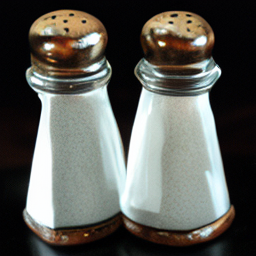
\includegraphics[width=0.12\textwidth]{samples/000001.png}
        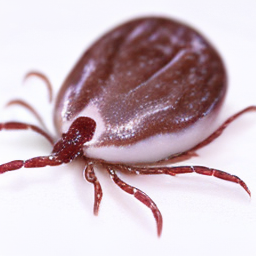
\includegraphics[width=0.12\textwidth]{samples/000002.png}
        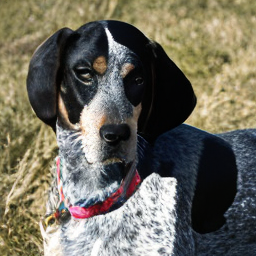
\includegraphics[width=0.12\textwidth]{samples/000003.png}
        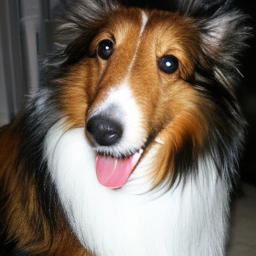
\includegraphics[width=0.12\textwidth]{samples/000004.png}
        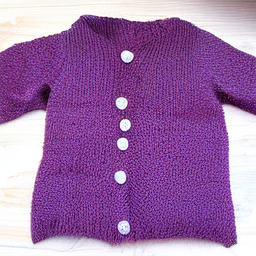
\includegraphics[width=0.12\textwidth]{samples/000005.png}
        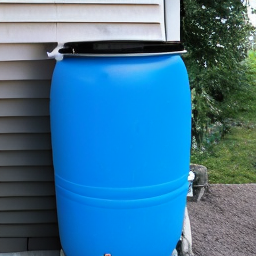
\includegraphics[width=0.12\textwidth]{samples/000006.png}
        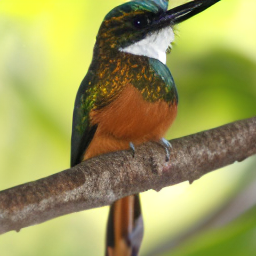
\includegraphics[width=0.12\textwidth]{samples/000007.png}
        
        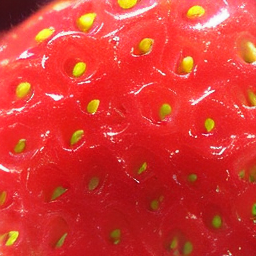
\includegraphics[width=0.12\textwidth]{samples/000008.png}
        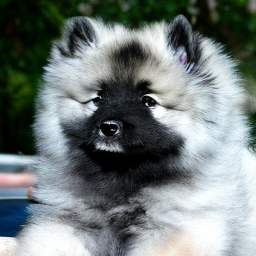
\includegraphics[width=0.12\textwidth]{samples/000009.png}
        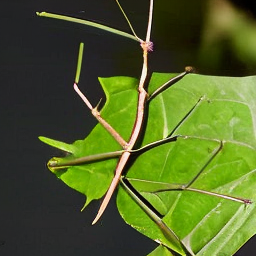
\includegraphics[width=0.12\textwidth]{samples/000010.png}
        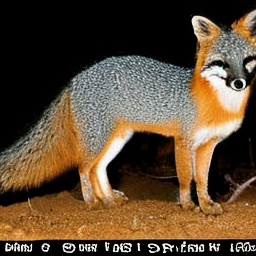
\includegraphics[width=0.12\textwidth]{samples/000011.png}
        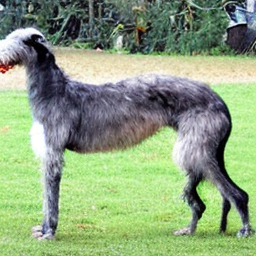
\includegraphics[width=0.12\textwidth]{samples/000012.png}
        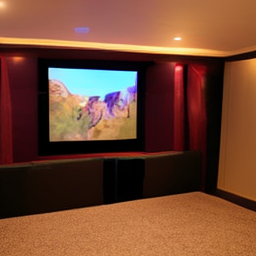
\includegraphics[width=0.12\textwidth]{samples/000013.png}
        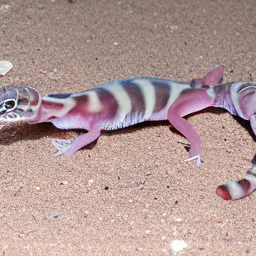
\includegraphics[width=0.12\textwidth]{samples/000014.png}
        
        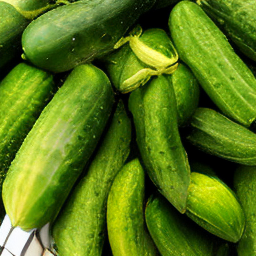
\includegraphics[width=0.12\textwidth]{samples/000015.png}
        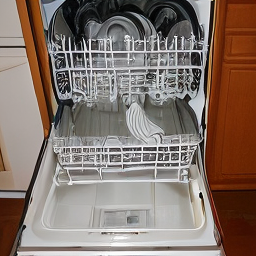
\includegraphics[width=0.12\textwidth]{samples/000016.png}
        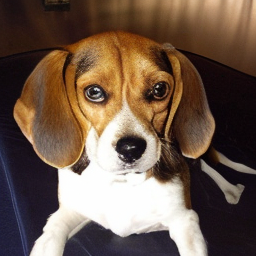
\includegraphics[width=0.12\textwidth]{samples/000017.png}
        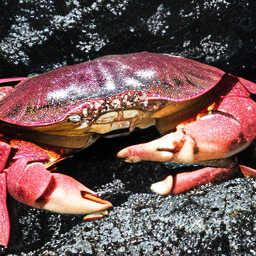
\includegraphics[width=0.12\textwidth]{samples/000018.png}
        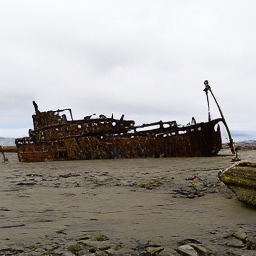
\includegraphics[width=0.12\textwidth]{samples/000019.png}
        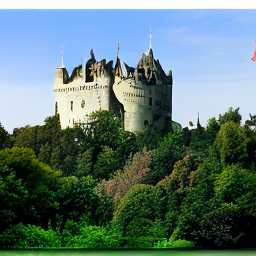
\includegraphics[width=0.12\textwidth]{samples/000020.png}
        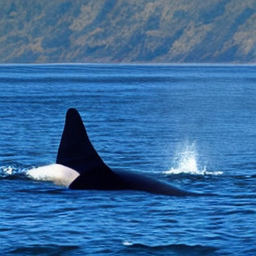
\includegraphics[width=0.12\textwidth]{samples/000021.png}
    \end{minipage}
    \caption{Selected images generated by SiT-L/2 model trained for 400K iterations with DINOv2-L as a target representation (with classifier guidance set to $4.0$). The presented samples demonstrate the diversity of outputs which can be produced by our trained models, as well as their shortcomings. For instance fine details are not resolved in some images, while others contain noise or structured artifacts such as the black banner with text-like shapes in the centre image.}
\end{figure*}

\subsection{Target Representation Experiment [Ondrej]}
We reproduced experiments comparing the effect of using different pre-trained self-supervised encoders as the target representation. The results are shown in Table~\ref{tab:target-representation}.

% \begin{tabular}{c c c c | c c c c c c | c c c c c}
% \toprule
% & & & & \multicolumn{6}{c|}{Theirs} & \multicolumn{5}{c}{Ours} \
% Iter. & Target Repr. & Depth
% & FID$\downarrow$ & sFID$\downarrow$ & IS$\uparrow$ & Pre.$\uparrow$ & Rec.$\uparrow$
% & FID$\downarrow$ & sFID$\downarrow$ & IS$\uparrow$ & Pre.$\uparrow$ & Rec.$\uparrow$ \
% \midrule
% 400K & \multicolumn{3}{c|}{Vanilla SiT-L/2~\cite{sit}}
% & 18.8 & 5.29 & 72.0 & 0.64 & 0.64
% & N/A & N/A & N/A & N/A & N/A \
% \hline
% 400K & MAE-L & 8
% & 12.5 & 4.89 & 90.7 & 0.68 & 0.63 
% & 15.06 & 5.27 & 85.37 & 0.66 & 0.63 \
% % 400K & DINO-B & 8 & NT-Xent
% % & 11.9 & 5.00 & 92.9 & 0.68 & 0.63 & 59.3
% % & N/A & N/A & N/A & N/A & N/A \
% 400K & MoCov3-L & 8
% & 11.9 & 5.06 & 92.2 & 0.68 & 0.64 
% & 16.08 & 5.29 & 82.85 & 0.65 & 0.64 \
% 400K & I-JEPA-H & 8 
% & 11.6 & 5.21 & 98.0 & 0.68 & 0.64
% & 10.27 & 5.36 & 111.53 &  0.68 & 0.65 \
% 400K & CLIP-L & 8 
% & 11.0 & 5.25 & 100.4 & 0.67 & 0.66
% & 10.61 & 5.28 & 107.61 & 0.69 & 0.65 \
% % 400K & SigLIP-L & 8
% % & 10.2 & 5.15 & 107.0 & 0.69 & 0.64
% % & N/A & N/A & N/A & N/A & N/A \
% 400K & DINOv2-L & 8 
% & 10.0 & 5.09 & 106.6 & 0.68 & 0.65
% & 9.73 & 5.30 & 112.80 & 0.69 & 0.65 \
% \bottomrule
% \caption{Target Representation Experiment on ImageNet 256×256. All models are SiT-L/2 trained for
% 400K iterations. We fix $\lambda=0.5$ as described in the paper. The $\downarrow$ and $\uparrow$ indicate whether lower or higher values are better, respectively.}
% \end{tabular}



\begin{table*}[t]
\centering
\begin{tabular}{ccc|ccccc|ccccc}
\toprule
& & & \multicolumn{5}{c|}{Theirs} & \multicolumn{5}{c}{Ours} \\
Iter. & Target Repr. & Depth
& FID$\downarrow$ & sFID$\downarrow$ & IS$\uparrow$ & Pre.$\uparrow$ & Rec.$\uparrow$
& FID$\downarrow$ & sFID$\downarrow$ & IS$\uparrow$ & Pre.$\uparrow$ & Rec.$\uparrow$ \\
\midrule
400K & \multicolumn{2}{c|}{Vanilla SiT-L/2~\cite{sit}}
& 18.8 & 5.29 & 72.0 & 0.64 & 0.64
& N/A & N/A & N/A & N/A & N/A \\
\hline
400K & MAE-L & 8
& 12.5 & 4.89 & 90.7 & 0.68 & 0.63
& 15.06 & 5.27 & 85.37 & 0.66 & 0.63 \\
400K & MoCov3-L & 8
& 11.9 & 5.06 & 92.2 & 0.68 & 0.64
& 16.08 & 5.29 & 82.85 & 0.65 & 0.64 \\
400K & I-JEPA-H & 8
& 11.6 & 5.21 & 98.0 & 0.68 & 0.64
& 10.27 & 5.36 & 111.53 & 0.68 & 0.65 \\
400K & CLIP-L & 8
& 11.0 & 5.25 & 100.4 & 0.67 & 0.66
& 10.61 & 5.28 & 107.61 & 0.69 & 0.65 \\
400K & DINOv2-L & 8
& 10.0 & 5.09 & 106.6 & 0.68 & 0.65
& 9.73 & 5.30 & 112.80 & 0.69 & 0.65 \\
\bottomrule
\end{tabular}
\caption{Target representation experiment on ImageNet at $256\times256$. All models are SiT-L/2 trained for 400K iterations. We fix $\lambda=0.5$ as described in the paper. Arrows indicate whether lower or higher values are better.}
\label{tab:repa-target-rep}
\label{tab:target-representation}
\end{table*}


We were unable to replicate experiments which use DINO-B and SigLIP-L as the target representation. In the case of DINO-B, the provided training script documents an approach for replicating their experiment, however the repository is missing crucial files required (\textit{models/dinov1.py}). We attempted substituting this file with the model file from the original repository of DINOv1\footnote{\href{https://github.com/facebookresearch/dino}{https://github.com/facebookresearch/dino}}, however training would require modifications to the training script, which we decided not to pursue, as this might not be a faithful reproduction of the original paper. In the case of SigLIP-L, the training script does not document how to replicate their experiment.   

\subsection{Target Encoder Depth [Frederik]}

The experiment testing effects of varying the depth at which the last-layer target representation from DINOv2-L is matched was reproduced. As in~\cite{yu2025repa}, we considered depths $d\in\{6,8,10,12,14,16\}$. The results of the experiment are presented in Table~\ref{tab:repa-depth}. Contrary to the results published in~\cite{yu2025repa}, $d=6$ fared better than $d=8$ in our reproduction. Nevertheless, our result corroborates the broader claim that representation matching depth has significant influence on training dynamics and downstream generation quality.

\begin{table*}[t]
    \centering
    \begin{tabular}{c c c | c c c c c | c c c c c}
        \toprule
              &              &           & \multicolumn{5}{c|}{Theirs} & \multicolumn{5}{c}{Ours} \\
        Iter. & Target Repr. & Depth & FID$\downarrow$ & sFID$\downarrow$ & IS$\uparrow$ & Pre.$\uparrow$ & Rec.$\uparrow$ & FID$\downarrow$ & sFID$\downarrow$ & IS$\uparrow$ & Pre.$\uparrow$ & Rec.$\uparrow$ \\
        \midrule
        400K & \multicolumn{2}{c|}{Vanilla SiT-L/2~\cite{sit}}
             & 18.8 & 5.29 & 72.00 & 0.64 & 0.64
             & N/A & N/A & N/A & N/A & N/A \\
        \hline
        400K & DINOv2-L & 6
             & 10.3 & 5.23 & 106.50 & 0.69 & 0.65
             & 9.3 & 5.24 & 118.10 & 0.69 & 0.65 \\
        400K & DINOv2-L & 8
             & 10.0 & 5.09 & 106.60 & 0.68 & 0.65
             & 10.0 & 5.27 & 112.23 & 0.68 & 0.65 \\
        400K & DINOv2-L & 10
             & 10.5 & 5.50 & 105.00 & 0.68 & 0.65
             & 10.0 & 5.30 & 112.70 & 0.68 & 0.65 \\
        400K & DINOv2-L & 12
             & 11.2 & 5.14 & 100.20 & 0.68 & 0.64
             & 10.7 & 5.37 & 108.70 & 0.68 & 0.66 \\
        400K & DINOv2-L & 14
             & 11.6 & 5.61 & 99.50 & 0.67 & 0.65
             & 11.0 & 5.37 & 106.90 & 0.68 & 0.65 \\
        400K & DINOv2-L & 16
             & 12.1 & 5.34 & 96.10 & 0.67 & 0.64
             & 12.1 & 5.42 & 100.30 & 0.67 & 0.65 \\
        \bottomrule
    \end{tabular}
    \caption{Results from the reproduced experiment of varying REPA alignment depth in SiT-L/2 using the last-layer output from DINOv2-L as the target representation.}
   
    \label{tab:repa-depth}
\end{table*}


\subsection{Model Size and Training Duration [Natasha]}

The experiment testing effects of varying learned model sizes (SiT-B/2 vs SiT-L/2 vs SiT-XL/2) and number of training epochs was reproduced, with results shown in Table~\ref{tab:tab-repa-size-epoch}. Our reproduction largely corroborates the findings in~\cite[Table~3]{yu2025repa}, with our numbers being the same or slightly worse (for SiT B/2) than what the reproduced paper reports. Larger models trained for a larger number of epochs exhibit better results. We did not train an SiT-XL/2 model for longer than 400K epochs due to time constraints, as reaching the latter number of epochs already exceeded 60 hours of training time. For comparison, only 25 hours were required to train an SiT-B/2 model for the same number of epochs.

A slight confusion arose when it came to determining which encoder was used for the target representation in~\cite{yu2025repa} for these experiments. The hyperparameters described in \cite[Table~7]{yu2025repa} claim that DINOv2-L was used for experiments with SiT-L/2 while DINOv2-B was used for experiments with SiT-B/2 and SiT-XL/2. We have some doubts whether this is accurate, as their reported FID of 9.7 (c.f. second row of Table~\ref{tab:tab-repa-size-epoch}) corresponds to DINOv2-B in~\cite[Table~2]{yu2025repa}.

Unfortunately, the description of the hyperparameters in the appendix of~\cite{yu2025repa} was not noted until after training had been carried out, so DINOv2-L was used in all experiments reported in Table~\ref{tab:tab-repa-size-epoch}. This may be a source of discrepancy with the results in~\cite{yu2025repa}, however we believe that any differences are small as supported by the ablation study on the effect of changing target encoder size (c.f. Section~\ref{sec:target-encoder-size}).

\begin{table*}[t]
    \centering
    \begin{tabular}{c c c | c | c c c c c}
    \toprule & & & Theirs & \multicolumn{5}{c}{Ours} \\
    Iter. & Model & Target Repr. & FID$\downarrow$ & FID$\downarrow$ & sFID$\downarrow$ & IS$\uparrow$ & Pre.$\uparrow$ & Rec.$\uparrow$ \\ \midrule
    400K & SiT-B/2 & DINOv2-L & 24.4 & 26.89 & 6.81 & 57.48 & 0.57 & 0.65 \\
    400K & SiT-L/2 & DINOv2-L & 9.7 & 10.01 & 5.27 & 112.23 & 0.68 & 0.65 \\
    700K & SiT-L/2 & DINOv2-L & 8.4 & 8.43 & 5.34 & 125.1 & 0.69 & 0.66 \\
    150K & SiT-XL/2 & DINOv2-L & 13.6 & 13.34 & 5.17 & 92.22 & 0.68 & 0.63 \\
    400K & SiT-XL/2 & DINOv2-L & 7.9 & 7.93 & 5.07 & 127.54 & 0.7 & 0.66 \\ \bottomrule \end{tabular}
    \caption{Results from reproduced experiments of varying REPA model size and training duration using the output from DINOv2-L as the target representation for layer 8.}
    \label{tab:tab-repa-size-epoch}
\end{table*}

WandB (Weights and Biases) was used to follow losses during training. The denoising loss (confusingly called ``loss'' in the logging) and the projection loss were recorded separately. A representative loss plot for training of SiT-XL/2 is shown in Figure~\ref{fig:sitxltraining}. Note that both losses fell continuously throughout the entire duration of training.

The gradual improvement of generated image quality was also observed using WandB by sampling a number of images every 10K epochs using classes fixed at the start of training for class-conditional generation. A series of images sampled for the ``lawn mower'' class throughout the training of our SiT-XL/2 model is presented in Figure~\ref{fig:sitxlwandbimages}, demonstrating gradual increase in quality.

\begin{figure*}
    \centering
    \begin{minipage}{\textwidth}
        \centering
        \includegraphics[width=0.11\textwidth]{assignment2/wandbsamples/image0.png}
        \includegraphics[width=0.11\textwidth]{assignment2/wandbsamples/image9999.png}
        \includegraphics[width=0.11\textwidth]{assignment2/wandbsamples/image19999.png}
        \includegraphics[width=0.11\textwidth]{assignment2/wandbsamples/image29999.png}
        \includegraphics[width=0.11\textwidth]{assignment2/wandbsamples/image39999.png}
        \includegraphics[width=0.11\textwidth]{assignment2/wandbsamples/image49999.png}
        \includegraphics[width=0.11\textwidth]{assignment2/wandbsamples/image59999.png}
        \includegraphics[width=0.11\textwidth]{assignment2/wandbsamples/image69999.png}
        
        \includegraphics[width=0.11\textwidth]{assignment2/wandbsamples/image79999.png}
        \includegraphics[width=0.11\textwidth]{assignment2/wandbsamples/image89999.png}
        \includegraphics[width=0.11\textwidth]{assignment2/wandbsamples/image99999.png}
        \includegraphics[width=0.11\textwidth]{assignment2/wandbsamples/image109999.png}
        \includegraphics[width=0.11\textwidth]{assignment2/wandbsamples/image119999.png}
        \includegraphics[width=0.11\textwidth]{assignment2/wandbsamples/image129999.png}
        \includegraphics[width=0.11\textwidth]{assignment2/wandbsamples/image139999.png}
        \includegraphics[width=0.11\textwidth]{assignment2/wandbsamples/image149999.png}
        
        \includegraphics[width=0.11\textwidth]{assignment2/wandbsamples/image159999.png}
        \includegraphics[width=0.11\textwidth]{assignment2/wandbsamples/image169999.png}
        \includegraphics[width=0.11\textwidth]{assignment2/wandbsamples/image179999.png}
        \includegraphics[width=0.11\textwidth]{assignment2/wandbsamples/image189999.png}
        \includegraphics[width=0.11\textwidth]{assignment2/wandbsamples/image199999.png}
        \includegraphics[width=0.11\textwidth]{assignment2/wandbsamples/image209999.png}
        \includegraphics[width=0.11\textwidth]{assignment2/wandbsamples/image219999.png}
        \includegraphics[width=0.11\textwidth]{assignment2/wandbsamples/image229999.png}
        
        \includegraphics[width=0.11\textwidth]{assignment2/wandbsamples/image239999.png}
        \includegraphics[width=0.11\textwidth]{assignment2/wandbsamples/image249999.png}
        \includegraphics[width=0.11\textwidth]{assignment2/wandbsamples/image259999.png}
        \includegraphics[width=0.11\textwidth]{assignment2/wandbsamples/image269999.png}
        \includegraphics[width=0.11\textwidth]{assignment2/wandbsamples/image279999.png}
        \includegraphics[width=0.11\textwidth]{assignment2/wandbsamples/image289999.png}
        \includegraphics[width=0.11\textwidth]{assignment2/wandbsamples/image299999.png}
        \includegraphics[width=0.11\textwidth]{assignment2/wandbsamples/image309999.png}
        
        \includegraphics[width=0.11\textwidth]{assignment2/wandbsamples/image319999.png}
        \includegraphics[width=0.11\textwidth]{assignment2/wandbsamples/image329999.png}
        \includegraphics[width=0.11\textwidth]{assignment2/wandbsamples/image339999.png}
        \includegraphics[width=0.11\textwidth]{assignment2/wandbsamples/image349999.png}
        \includegraphics[width=0.11\textwidth]{assignment2/wandbsamples/image359999.png}
        \includegraphics[width=0.11\textwidth]{assignment2/wandbsamples/image369999.png}
        \includegraphics[width=0.11\textwidth]{assignment2/wandbsamples/image379999.png}
        \includegraphics[width=0.11\textwidth]{assignment2/wandbsamples/image389999.png}     
    \end{minipage}
    \caption{Images for ``lawn mower'' class sampled with CFG=4 every 10K epochs during training of our SiT-XL/2 (c.f. Table~\ref{tab:tab-repa-size-epoch})}
    \label{fig:sitxlwandbimages}
\end{figure*}


\begin{figure}
    \centering
    \includegraphics[width=0.9\linewidth]{assignment2/graphs/sitxl_proj_loss.png}
    \vspace{0.5em}
    \includegraphics[width=0.9\linewidth]{assignment2/graphs/diffusionloss_sit_xl.png}
    \caption{Projection (upper) and Diffusion (lower) losses exhibited by SiT-XL/2 trained for 400K epochs with DINOv2-L as target representation and $\lambda = 0.5$ (c.f. Table~\ref{tab:tab-repa-size-epoch})}
    \label{fig:sitxltraining}
\end{figure}

\subsection{Artifacts}

Our trained models and images generated for evaluation are available online and can be downloaded from \href{https://sharepoint.markmizzi.com/atdl-assignment-2/models}{this link}. See the \href{https://github.com/MarkMizzi/ADTL-Assignment-2#artifacts}{README} in \cite{mainrepo} for more details.

\section{Discussion}\label{sec:discussion}
Across all experiments, we were able to achieve comparable, but not equal, performance to the results of the reproduced paper. 

Our replication of experiments comparing the impact of different target representation encoder sizes of various DINOv2 models, shown in Table \ref{tab:tab-repr-target-size} confirmed that the difference in performance across encoder sizes is in fact marginal, supporting the findings of the authors. 

Investigation of different pre-trained self-supervised encoders (c.f. Table \ref{tab:repa-target-rep}) is largely consistent with the paper's findings in terms of relative performance. In our experiments, the model with  I-JEPA-H as its target encoder achieved the most significant increase, while the MoCov3-L encoder showed a decrease in performance. We hypothesize that these differences in results are primarily caused by the objective function used during training. The results in the paper were obtained using an NT-Xent objective, whereas our training was conducted with cosine similarity, due to the fact that the training script provided by the authors implements only the latter (c.f. Section~\ref{sec:scope}). We opted for this approach as it did not require large changes to the original source code, allowing us to closely mimic the approach of the authors. The authors justify not including the NT-Xent objective by  empirically observing that the gap between these two approaches diminishes over time; however our experiments show this does not hold uniformly across all encoder types.

The impact of depth at which the last layer target representation from DINOv2-L is matched is shown in Table~\ref{tab:repa-depth}. In our experiments models generally exhibited improved  performance compared to~\cite{yu2025repa} for all layers, with the biggest improvements observed for layers 6 and 14. Importantly, our results align with the observation that regularizing only the first few layers (8,6) is sufficient and enhances generation performance. Again, we attribute the improvement to our use of cosine similarity as an objective, as this was the only differing factor.

Our last set of reproduced experiments which test effects of model size and training duration (c.f. Table~\ref{tab:tab-repa-size-epoch}) confirms that performance continues to improve with more epochs and bigger vanilla SiTs. We hypothesize that any differences in our results is a result of our usage of DINOv2-L rather than DINOv2-B, however as both our experiments confirm (c.f. Table~\ref{tab:tab-repr-target-size}), the difference between these two encoders is marginal.

\section{Conclusion}\label{sec:conclusion}
Our work validates the main premise of~\cite{yu2025repa}, namely that representation alignment at particular intermediate hidden layers is conducive to an increase in image generation quality relative to the baseline of no alignment. Moreover, we replicated several of the trends observed in~\cite{yu2025repa}, although our results differ slightly which is to be expected given minor differences in our experimental setup, such as training with a different auxiliary matching loss.

\section{Individual Contributions}

Each team member was responsible for reproducing an experiment from~\cite{yu2025repa}, as indicated in the text above. Mark was responsible for setting up the Github repositories/sharepoint, pre-processing the training dataset and writing training tutorials for the rest of the team. Writing tasks were split as follows: the abstract and conclusion were authored by Frederik, Section~\ref{sec:theory} by Natasha, Sections~\ref{sec:scope},~\ref{sec:experiments} by Mark, and Section~\ref{sec:discussion} by Ondrej. The results reported in Section~\ref{sec:results} were described by the person who conducted each experiment.


\bibliographystyle{IEEEbib}
\bibliography{strings,refs}

\end{document}
